\ifmidterm
\chapter{Preliminary Results\sv{Preliminära resultat}}
\else
\chapter{Results\sv{Resultat}}
\fi
\label{chap:results}
\begin{instructions}
Tell the reader, in an objective way, without judgements or analysis, what you have achieved\onlyin{midterm}{ so far}.
\begin{onlyfinal}
Most importantly, you should include the results of the tests you described in Section~\ref{sec:devprocess} and~\ref{sec:deployment}. Include how you proceeded to conduct the tests:
\begin{itemize}
    \item both for the components of your architecture and the complete artifact (see Section~\ref{sec:techdesign}). \textcolor{red}{If applicable, also for the integration with a larger system}
    \item both the functional and the non-functional requirements (see Section~\ref{sec:req})
\end{itemize}
\end{onlyfinal}

Typically this section will include tables and images. Here is how to do tables. They will appear automatically in the list of tables.
\begin{table}[ht]
  \centering
  \caption{A simple, manually formatted example table}
  \label{tab:example1}
  \begin{tabular}{cc}
    \hline
    age  & IQ \\
    \hline
    10   & 110 \\
    20   & 120 \\
    30   & 145 \\
    40   & 120 \\
    50   & 100 \\
    \hline
  \end{tabular}
\end{table}

\begin{table}[ht]
  \centering
  \caption[A simple example table generated from a CSV file]{A simple example table generated from a CSV file using \texttt{simplecsv} and \texttt{booktab}}
  \label{tab:examplecsv}
  \csvautobooktabular{csvtables/ageiq.csv}
\end{table}

Here, you can see how to introduce an image in a figure. The picture shown in Figure~\ref{fig:lion} is merely for decorative purposes and shows a cartoon of a lion winking while handling books.

\begin{figure}[htbp]  % order of priority: h here, t top, b bottom, p page
  \centering
  
\includegraphics[width=.5\textwidth]{figures/lion.png}
  \caption[The \LaTeX{} logotype]{The \LaTeX{} logotype}
  \label{fig:lion}
\end{figure}

You can refer to it as Figure~\ref{fig:lion} and in this template it is very likely that it ends up on the \emph{next page}. \emph{Please observe:} \LaTeX{} has very good reasons to put figures where they are put after you compile your work. Don't fight it, it will not be worth the effort. Instead, be very specific in your text what the figure describes and refer to it properly.
It appears automatically in the list of figures.

If you want to create figures with data directly in the report file, PGFPLOTS and TIKZ can be used. Figure~\ref{fig:iq-plot}  shows the data from Table~\ref{tab:example1} plotted as a scatter plot exemplifying this.

\begin{figure}[htbp]  % order of priority: h here, t top, b bottom, p page
  \centering
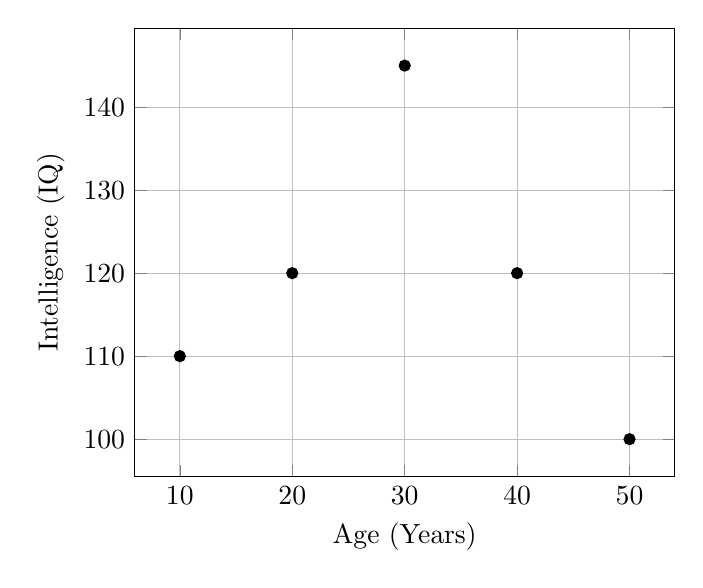
\begin{tikzpicture}
    \begin{axis}[
        xlabel={Age (Years)},
        ylabel={Intelligence (IQ)},
        grid=major
    ]
    \addplot[only marks] table {
        x y
        10 110
        20 120
        30 145
        40 120
        50 100
    };
    \end{axis}
\end{tikzpicture}
  \caption{A simple scatterplot generated from text data in the report.}
  \label{fig:iq-plot}
\end{figure}
\end{instructions}
